\setcounter{chapter}{2}
\chapter{Cơ sở lý thuyết}

Ở chương này, tôi tập trung vào việc giới thiệu các thuật toán, mô hình, các độ đo hoặc công nghệ mà tôi sử dụng trong đồ án và đi sâu về mặt lý thuyết.
\section{Mô hình CRF}
CRF (Conditional Random Fields) - Trường ngẫu nhiên có điều kiện là một mô hình dựa trên xác suất có điều kiện, là một dạng của mô hình phân biệt (Discriminative model), thường được sử dụng trong các bài toán dự đoán cấu trúc, gán nhãn dữ liệu dạng chuỗi tuần tự (Sequences Tagging).
\subsection{Discriminative classifier}
Các mô hình học máy nhìn chung thường được phận loại thành 2 dạng chính, đó là \textit{Generative model (Mô hình sinh)} và \textit{Discriminative model (Mô hình phân biệt)}. CRF là một loại của Discriminative model, và do đó, chúng mô hình hóa ranh giới quyết định giữa các lớp khác nhau. Generative model, theo một cách khác, chúng mô hình hóa cách dữ liệu được sinh ra và sau khi được huấn luyện, mô hình có thể được sử dụng như một bộ phân loại.

Một ví dụ đơn giản và phổ biến của bộ phân loại theo xác suất là Naive Bayes - một bộ phân loại dựa trên Maximum Likelihood Estimation (MLE), là một Discriminative model.

Bộ phân loại Naive Bayes dựa trên giải thuật Naive Bayes, có công thức tổng quát:

$$ P(y \mid X) = \frac{P(X \mid y) \, P(y)}{P(X)} $$
\begin{center}

\vspace{0.3cm}
\textbf{3.1.} \textit{Công thức Bayes}    
\end{center}

Dự đoán mà bộ phân loại đưa ra, có thể được biểu diễn dưới dạng xác suất có điều kiện, và có thể được phân tách bằng giải thuật Naive Bayes:

Giả sử ta có các điểm dữ liệu ${\textbf{x}_1}$, ${\textbf{x}_2}$, ${\textbf{x}_3}$,.., ${\textbf{x}_n}$. Giả sử thêm rằng ta đã biết các điểm dữ liệu này tuân theo một phân phối nào đó được mô tả bởi bộ tham số\textit{y}.
Dựa trên giả định các điểm dữ liệu là độc lập, ta có :
$$ P({\textbf{x}_1}, {\textbf{x}_2}, {\textbf{x}_3},.., {\textbf{x}_n} \mid y) \approx \prod_{n=1}^{N} P({\textbf{x}_n} \mid y)$$
\begin{center}

\vspace{0.3cm}
\textbf{3.2.} \textit{Công thức xấp xỉ theo giả định các điểm dữ liệu là độc lập }       
\end{center}

Thay vào \textbf{3.1} ta được :
$$ P(y \mid X) \approx \frac{\prod_{n=1}^{N} P({\textbf{x}_n} \mid y) \, P(y)} {P({\textbf{x}_1}, {\textbf{x}_2}, {\textbf{x}_3},.., {\textbf{x}_n})} $$
\begin{center}

\vspace{0.3cm}
\textbf{3.3.} \textit{Công thức Bayes theo giả định độc lập}    
\end{center}

Bởi vì mẫu số là hằng số, nên ta có thể rút gọn:
$$ P(y \mid X) \approx \prod_{n=1}^{N} P({\textbf{x}_n} \mid y) \, P(y)$$
\begin{center}

\vspace{0.3cm}
\textbf{3.4.} \textit{Công thức Bayes rút gọn theo giả định độc lập}    
\end{center}
Bài toán trở thành bài toán tối ưu y sao cho xác suất $P(y \mid X)$ đạt cực đại:
$$\Hat{y} = argmax_y \prod_{n=1}^{N} P({\textbf{x}_n} \mid y) \, P(y)$$

\begin{center}

\vspace{0.3cm}
\textbf{3.5.} \textit{Công thức tối ưu tham số theo MLE }    
\end{center}

Trên đây là một ví dụ về cách bộ phân loại Naive Bayes, là một bộ phân loại thuộc Discriminative model, tối ưu các tham số dựa trên MLE.
\subsection{Conditional Random Fields (CRF)}
Để thuận tiện cho việc trình bày, trong phần này, tôi sẽ sử dụng kí hiệu $\underline{w}$ thay cho vector có các thành phần $w_1, w_2,...w_d$, sử dụng $\exp(x)$ thay cho $e^x$. 

% \subsubsection{Feature Function}
% Mô hình CRF nhận dữ liệu đầu vào là chuỗi tuần tự (sequential), khi dự đoán về một điểm dữ liệu, thì mô hình thường quan tâm đến các ngữ cảnh trước đó. Để mô hình hóa hành vi này, CRF sử dụng các \textit{Feature Function} mà có thể nhận nhiều giá trị đầu vào, có thể là :

% \hspace{1cm}  - một câu s

% \hspace{1cm}  - vị trí i của một từ trong câu s

% \hspace{1cm}  - nhãn ${l_i}$ của từ hiện tại 

% \hspace{1cm}  - nhãn ${l_{i-1}}$ của từ liền trước 

% \vspace{0.3cm}
% Một \textit{Feature Function} có thể được định nghĩa như sau: \newpage
% $$f(s,i,{l_i},{l_{i-1}})$$
% \begin{center}
% \textbf{3.6.} \textit{Ví dụ về \textit{Feature Function} }    
% \end{center}

% Đầu ra của các \textit{Feature Function} là một số thực (thường nằm trong khoảng từ 0 đến 1).

% Mục đích của các \textit{Feature Function} là để mô tả một số đặc tính mà các điểm dữ liệu biểu diễn. Một ví dụ về bài toán gãn nhán từ loại sử dụng CRF có \textit{Feature Function} :

% \vspace{0.2cm}
% $f (X, i, L_{i-1}, L_{i} ) = \textbf{1}$ Nếu $L_{i-1}$ là danh từ, và $L_i$ là động từ, còn lại bằng \textbf{0}

% \vspace{0.2cm}
% Tương tự, có thể có :

% \vspace{0.2cm}
% $f (X, i, L_{i-1}, L_{i} ) = \textbf{1}$ Nếu $L_{i-1}$ là động từ, và $L_i$ là trạng từ, còn lại bằng \textbf{0}

% \vspace{0.2cm}
% Mỗi \textit{Feature Function} phụ thuộc vào nhãn của từ hiện tại và từ liền trước nó, có thể nhận giá trị 0 hoặc 1. Ví dụ một \textit{Feature Function} có khả năng ước lượng được liệu một từ có phải là tính từ hay không nếu từ đứng trước nó là \textit{very}.

% Để có thể xây dựng được mô hình, mỗi \textit{Feature Function} $f_i$ được gán một trọng số  $\lambda_{i}$ để biểu diễn mức độ quan trọng của các \textit{Feature Function} với mô hình trên tập dữ liệu.

% Giả sử có một câu s, ta có thể tính điểm cho một nhãn l của s bằng cách thêm trọng số $\lambda_{i}$ cho tất cả các từ của câu s:
% $$score(l \mid s) = \sum_{j=1}^{m} \sum_{i=1}^{n}\lambda_{j}f_{j} (s, i, l_{i-1}, l_{i} )$$
% \begin{center}

% \vspace{0.3cm}
% \textbf{3.7.} \textit{Công thức tính score cho một nhãn l của câu s }    
% \end{center}

% Biến đối về dạng xác suất có điều kiện :

% $$P(l \mid s) = \frac{exp[score(l\mid s)]}{\sum_{l'}exp[score(l' \mid s)]} = \frac{exp[\sum_{j=1}^{m} \sum_{i=1}^{n}\lambda_{j}f_{j} (s, i, l_{i-1}, l_{i} )]}{\sum_{l'}exp[\sum_{j=1}^{m} \sum_{i=1}^{n}\lambda_{j}f_{j} (s, i, l'_{i-1}, l'_{i} )]}$$

% \begin{center}

% \vspace{0.3cm}
% \textbf{3.8.} \textit{Công thức tính xác suất cho một nhãn l của câu s }    
% \end{center}

% Để có thể xây dựng được CRF, chúng ta cần định nghĩa các \textit{Feature Function}, có thể dựa vào các yếu tố như: phân biệt chữ hoa, chữ thường trong câu, vị trí của từ trong câu, từ là số hay là chữ,... Tất cả những yếu tố này được lựa chọn phụ thuộc vào bộ dữ liệu chúng ta huấn luyện và kết quả mà chúng ta muốn hướng tới.

% \subsubsection{Tối ưu tham số}
% Để ước lượng được tham số  feature weights ($\lambda_{i}$) trong một mô hình CRF, chúng ta sẽ sử dụng \textit{Gradient Descent}.

% Giả sử chúng ta có một tập dữ liệu huấn luyện (gồm các câu đã được gán nhãn từng từ). Khởi tạo ngẫu nhiên một vector trọng số, sau đó ta sẽ đi tối ưu vector trọng số này.
% \newpage
% Vòng lặp:
%một vector trọng số $\underline{\textit{w}}$ \in $\mathbb{R}^{d}$
\subsubsection{Log-linear models}
Giả sử có hai tập $\textbf{X}$ và $\textbf{Y}$, tập \textbf{Y} là tập hữu hạn. Mục tiêu của chúng ta là xây dựng một mô hình để ước lượng xác suất có điều kiện $p(y\mid x)$ là xác suất của một nhãn $y \in \textbf{Y}$ với đầu vào là $x \in \textbf{X}$. Ví dụ với bài toán gán nhãn từ loại, $x$ có thể là một từ, $y$ có thể là các nhãn N (danh từ), V (động từ),... Một feature-vector $\underline{\phi}: \textbf{X} \times \textbf{Y} \longrightarrow \mathbb{R}^d $, một vector trọng số $\underline{w} \in \mathbb{R}^{d}$. Log-liner models được định nghĩa với công thức như sau:
$$p(y \mid x; \underline{w}) = \frac{exp(\underline{w} \cdot \underline{\phi}(\textit{x,y}))}{\sum_{\textit{y'} \in \textbf{Y}} exp(\underline{w} \cdot \underline{\phi}(\textit{x,y'}))} $$
\begin{center}

\vspace{0.3cm}
\textbf{3.6.} \textit{Công thức log-linear models}    
\end{center}
Đây là xác suất có điều kiện của y khi biết đầu vào x, với tham số $\underline{w}$.
Tích số 
$$\underline{w}\cdot \underline{\phi}(\textit{x,y})$$
\begin{center}

\vspace{0.3cm}
\textbf{3.7.} \textit{Tích trọng số và feature-vector}    
\end{center}
có thể nhận giá trị dương hoặc âm, có thể được coi như một định lượng về mức độ hợp lý của nhãn \textit{y} với đầu vào \textit{x}. Với một đầu vào \textit{x}, ta có thể tính toán được tích số \textbf{3.7} với mỗi nhãn $\textit{y} \in \textbf{Y}$. Để có thể chuyển về dạng phân phối xác suất một cách chính xác, tích số \textbf{3.7} phải luôn dương. Do đó ta sẽ sử dụng hàm exp():
$$exp(\underline{w}\cdot \underline{\phi}(\textit{x,y}))$$
Giá trị này luôn lớn hơn 0. Cuối cùng, chuẩn hóa bằng cách chia cho tổng của tất cả tích số \textbf{3.7} trên tất cả các nhãn
$$\sum_{\textit{y'} \in \textbf{Y}} exp(\underline{w} \cdot \underline{\phi}(\textit{x,y'}))$$
ta có thể đảm bảo rằng xác suất  $p(y \mid x; \underline{w})$ luôn nằm trong khoảng $[0;1]$ dù tích số \textbf{3.7} có thể nhận giá trị âm hoặc dương.

\textbf{Log-Likelihood Function}
Trong phần trước, tôi đã đề cập đến việc tối ưu tham số cho bộ phân loại Naive Bayes bằng MLE. Trong phần này, tôi sẽ trình bày chi tiết hơn về cách MLE tối ưu tham số.

Giả sử ta có một tập gồm n điểm dữ liệu, $\{(x_i,y_i)\}_{i=1}^{n}$. Log-likehood function được định nghĩa là:

$$L(\underline{w}) = \sum_{i=1}^{n}\log p(y_i\mid x_i; \underline{w})$$
\begin{center}

\vspace{0.3cm}
\textbf{3.8.} \textit{Log-likelihood function}    
\end{center}
Chúng ta có thể hiểu $L(\underline{w})$ là một hàm mà với một giá trị \underline{w} cho trước, ta có thể đo được \underline{w} mô tả dữ liệu tốt như thế nào. Ví dụ, một giá trị \underline{w} tốt sẽ cho giá trị $p(y_i \mid x_i; \underline{w})$ cao với mọi \textit{i} = 1...n, và do vậy chúng ta cũng có một giá trị $L(\underline{w})$ cao.

Maximum-likelihood estimates là đi tìm một giá trị $\underline{w}$ để cực đại hóa xác suất $p(y_i\mid x_i ; \underline{w})$ hay "khớp" nhất với bộ dữ liệu huấn luyện dựa trên tiêu chí $L(\underline{w})$:

$$\underline{w}^* = \arg \max_{\underline{w} \in \mathbb{R}^d} \sum_{i=1}^n \log p(y_i \mid x_i; \underline{w})$$

\begin{center}

\vspace{0.3cm}
\textbf{3.9.} \textit{Công thức tối ưu tham số MLE}    
\end{center}

Để có thể giải quyết bài toán MLE, chúng ta sử dụng \textit{Gradient Decent} và sau khi tính toán sẽ thu được tham số $\underline{w}^T$ là một tham số tối ưu của mô hình.

\vspace{0.3cm}
\textbf{Regularized log-likelihood}
Trong nhiều ứng dụng đã được kiểm chứng là đạt hiệu quả cao, log-likelihood thường được thêm vào một số \textit{regularization term}, khi đó log-likelihood trở thành :
$$L(\underline{w}) = \sum_{i=1}^{n}\log p(y_i\mid x_i; \underline{w}) - \frac{\lambda}{2}\| \underline{w}\|^2$$
Trong đó, $\|\underline{w}\|^2 = \sum_j w^2_j$ và $\lambda > 0$,
việc giải quyết bài toán vẫn là đi tìm $\underline{w}$ sao cho $L(\underline{w})$ đạt cực đại.
$$\underline{w}^* = \arg \max_{\underline{w} \in \mathbb{R}^d} L(\underline{w})$$
Tương tự như trong phần log-likelihood, ta vẫn sử dụng \textit{Gradient Descent} để tìm ra giá trị $\underline{w}^*$ tối ưu cho bài toán.

\subsubsection{CRFs model}
Trong phần này, tôi cũng sẽ sử dụng $\underline{x}$ thay cho một chuỗi đầu vào $x_1 ... x_m$, và $\underline{s}$ thay cho một chuỗi các trạng thái $s_1 ... s_m$. Tập hợp các trạng thái có thể xảy ra là $S$. Tập hợp tất cả các chuỗi trạng thái có thể có là $S^m$. 

Trong CRFs, chúng ta sẽ xây dựng lại một model của $$p(s_1 ... s_m\mid x_1 ... x_m) = p(\underline{s}\mid \underline{x})$$

Đầu tiên, CRFs sẽ định nghĩa một feature vector
$$ \underline{\Phi}(\underline{x},\underline{s}) \in \mathbb{R}^d$$
vector này sẽ ánh xạ toàn bộ chuỗi đầu vào $\underline{x}$ với toàn bộ chuỗi trạng thái $\underline{s}$ tương ứng theo cặp thành một số feature vector $d$ chiều .Feature vector này được định nghĩa như sau:
$$\underline{\Phi}(\underline{x},\underline{s}) = \sum_{j=1}^m \underline{\phi}(\underline{x},j,s_{j-1},s_j)$$
\begin{center}

\vspace{0.2cm}
\textbf{3.10.} \textit{Công thức feature vector}    
\end{center}
Trong đó :
\begin{itemize}
    \item $\underline{x}$ là toàn bộ câu đang xét
    \item $i$ là vị trí được gắn thẻ (giá trị từ 1 đến $m$)
    \item $s_{j-1}$ là giá trị trạng thái liền trước của trạng thái hiện tại(có thể là bất kì giá trị nào trong $S$)
    \item $s_j$ là giá trị trạng thái mới(có thể là bất kì giá trị nào trong $S$)
\end{itemize}

Giả sử có 1 feature thứ k nào đó trong khoảng 1 ... d, feature vectore tại k sẽ là:
$$\Phi_k(\underline{x},\underline{s}) = \sum_{j=1}^m \phi_k(\underline{x},j,s_{j-1},s_j)$$
\begin{center}

\vspace{0.1cm}
\textbf{3.11.} \textit{Công thức feature vector tại một giá trị $k$ bất kì}    
\end{center}
Từ đó, ta có thể tính được giá trị $\Phi_k$ bằng cách tính tổng của tất cả các $\phi_k$ trên toàn bộ $m$ trạng thái khác nhau từ $s_1...s_m$

Sau đó chúng ta sẽ xây dựng log-linear model,
$$p(\underline{s}\mid \underline{x};\underline{w}) = \frac{\exp (\underline{w} \cdot \underline{\Phi}(\underline{x},\underline{s})}{\sum_{\underline{s'}\in S^m } \exp (\underline{w} \cdot \underline{\Phi}(\underline{x},\underline{s'})}$$

\begin{center}

\vspace{0.1cm}
\textbf{3.12.} \textit{Công thức log-linear model cho CRFs}    
\end{center}

Đây là một công thức cần lượng tính toán rất lớn, do không gian các giá trị có thể xảy ra với $\underline{s}$ là $S^m$, vô cùng lớn, và việc tính toán tổng ở dưới mẫu trong \textbf{3.12} cũng bị lặp lại nhiều lần. Tuy nhiên nếu đưa ra các giả định thích hợp, ta có thể huấn luyện và tính toán mô hình này một cách khá hiệu quả.

\vspace{0.3cm}
\textbf{Decoding với CRFs} Vấn đề này được phát biểu như sau: Cho một chuỗi đầu vào $\underline{x} = x_1, x_2, ... x_m$, chúng ta phải tìm ra được một chuỗi trạng thái thích hợp nhất với chuỗi đầu vào theo mô hình 
$$\arg max_{\underline{s} \in S^m} p(\underline{s}\mid \underline{x}; \underline{w})$$

Biến đổi dựa vào \textbf{3.10} thu được:
$$\arg max_{\underline{s} \in S^m} p(\underline{s}\mid \underline{x}; \underline{w}) = \arg \max_{\underline{s} \in S^m} \sum_{j=1}^m \underline{w} \cdot \underline{\phi}(\underline{x},j,s_{j-1},s_j)$$

Giải quyết vấn đề decoding chính là đi tìm một chuỗi trạng thái sao cho cực đại hóa:
$$\arg \max_{\underline{s} \in S^m} \sum_{j=1}^m \underline{w} \cdot \underline{\phi}(\underline{x},j,s_{j-1},s_j)$$

Mỗi khi chuyển trạng thái từ $s_{j-1}$ sang $s_j$ đều có một số điểm liên kết:
$$\underline{w} \cdot \underline{\phi}(\underline{x},j,s_{j-1},s_j)$$

Để giải bài toán này, ta sử dụng biến thể của giải thuật Viterbi
\begin{itemize}
    \item Khởi tạo : for $s \in S$
    $$\pi[1,s] = \underline{w} \cdot \underline{\phi}(\underline{x},1,s_0,s)$$
    $s_0$ là một giá trị khởi tạo đặc biệt "initial"
    \item For $j = 2 ... m, s = 1 ... k$ :
    $$\pi[j,s] = max_{s' \in S}[\pi [j-1,s'] + \underline{w} \cdot \underline{\phi}(\underline{x},j,s',s)]$$
\end{itemize}

Cuối cùng ta được :
$$ \max_{s1 ... sm} \sum_{j=1}^m \underline{w} \cdot \underline{\phi}(\underline{x},j,s_{j-1},s_j) = \max_{s}\pi[m,s]$$
\begin{center}

\vspace{0.1cm}
\textbf{3.13.} \textit{Công thức decoding trong CRFs}    
\end{center}

Thuật toán này chỉ chạy với độ phức tạp là $O(mk^2)$ nên việc decodeing trong CRFs là hoàn toàn khả thi.

\vspace{0.5cm}
\textbf{Ước lượng tham số trong CRFs} Để ước lượng tham số, giả sử ta có một tập dữ liệu gồm n ví dụ đã được gán nhãn $\{(\underline{x}^i,\underline{s}^i)\}_{i=1}^n$. Mỗi $\underline{x}^i$ là một chuỗi đầu vào $x_1^i ... x_m^i$, mỗi $\underline{s}^i$ là một chuỗi các trạng thái $s_1^i ... s_m^i $. Việc tối ưu tham số được thực hiện giống như ở phần \textit{regular log-linear models}:
$$L(\underline{w}) = \sum_{i=1}^n \log p(\underline{s}^i \mid \underline{x}^i;w) - \frac{\lambda}{2}\|\underline{w}\|^2$$

Tham số $\underline{w}$ được ước lượng:
$$\underline{w}^* = \arg \max_{\underline{w} \in \mathbb{R}^d} \sum_{i=1}^n \log p(\underline{s}^i \mid \underline{x}^i; \underline{w}) - \frac{\lambda}{2}\|\underline{w}\|^2 $$
\begin{center}

\vspace{0.1cm}
\textbf{3.14.} \textit{Công thức tối ưu tham số trong CRFs}    
\end{center}

Để tìm ra được giá trị $\underline{w}^*$, \textit{Gradient Descent} vẫn là sự lựa chọn tối ưu, về chi tiết của giải thuật, tôi không trình bày chi tiết vì trong chương này tôi chỉ muốn giới thiệu cơ bản về các mô hình và công nghệ mà tôi sử dụng.

\section{Máy tìm kiếm}
Ở phần này, tôi sẽ trình bày về các công nghệ cốt lõi mà phương pháp Sagel sử dụng. Về cơ bản, giải thuật của Sagel là một giải thuật \textit{Fuzzy Matching}, giải thuật này cần phải \textit{match} chuỗi địa chỉ đầu vào với một chuỗi địa chỉ trong hàng chục nghìn, thậm chí là hàng trăm nghìn chuỗi địa chỉ chuẩn. Vì vậy, việc đảm bảo tốc độ là vô cùng cần thiết. Máy tìm kiếm là một lựa chọn tối ưu.

\vspace{0.5cm}
\textbf{Máy tìm kiếm}, tên gọi tiếng Anh là \textit{Search Engine}, là một hệ thống truy vấn thông tin, các kết quả trả về thường được biểu diễn trong một danh sách, và được gọi là \textit{hits}. Máy tìm kiếm được xây dựng và thiết kế để giảm thiểu thời gian cần thiết trong quá trình truy vấn. Trong phạm vi của đồ án, tôi sử dụng máy tìm kiếm \textit{Elasticsearh}, là một máy tìm kiếm phố biến hiện nay. Ở trong \textit{section} này, tôi sẽ tập trung giới thiệu về \textit{Elasticsearh}. 
\subsection{Chỉ mục ngược}
\textit{Elasticsearch} sử dụng một cấu trúc gọi là \textit{chỉ mục ngược} hay \textit{invered index}. Chỉ mục này được thiết kế để cho phép thực hiện các truy vấn \textit{full-text} với tốc độ rất cao. Dưới đây là một ví dụ về chỉ mục ngược:
\vspace{0.3cm}

1. Tôi học tại trường Bách Khoa Hà Nội

2. Bách Khoa thật đẹp
\vspace{0.3cm}

Có 2 văn bản có chứa các từ như trên, gọi là doc\_1 và doc\_2. Chỉ mục ngược sẽ không lưu trữ theo thông thường là doc - words mà lưu trữ ngược theo theo dạng word - docs. Đây là lí do vì sao nó được đặt tên là chỉ mục ngược hay chỉ mục đảo.

Với ví dụ trên, kết quả sẽ như sau:
\begin{center}
\begin{tabular}{||c c c||} 
 \hline
 term & doc\_1 & doc\_2 \\ [0.5ex] 
 \hline\hline
Tôi   &    X  &   \\
học     &   X   & \\
tại   &   X   &   \\
trường     &   X   & \\
Bách   &    X   &  X \\
Khoa    &   X   &  X\\
Hà   &      X  &  \\
Nội      &   X    &  \\
thật  &      &  X\\
đẹp    &      &  X \\[1ex] 
 \hline
\end{tabular}
\end{center}

\begin{center}

\vspace{0.1cm}
\textbf{Bảng 1.} \textit{Ví dụ về chỉ mục ngược}    
\end{center}

Với 1 truy vấn \textit{Tôi đến Bách Khoa}, máy tìm kiếm chỉ cần tìm văn bản có xuất hiện các từ \textit{Tôi}, \textit{đến}, \textit{Bách}, \textit{Khoa}. Trong trường hợp này, doc\_1 xuất hiện 3 từ \textit{Tôi, Bách, Khoa}, doc\_2 xuất hiện 2 từ \textit{Bách, Khoa}. Hai văn bản này đều liên quan đến câu truy vấn, tuy nhiên doc\_1 sẽ được cho điểm số cao hơn là doc\_2 do chứa nhiều từ hơn.
\begin{center}
\begin{tabular}{||c c c||} 
 \hline
 term & doc\_1 & doc\_2 \\ [0.5ex] 
 \hline\hline
Tôi   &    X  &   \\
đến     &      & \\
Bách   &    X   &  X \\
Khoa    &   X   &  X\\[1ex]
 \hline
\end{tabular}
\end{center}
\begin{center}

\vspace{0.1cm}
\textbf{Bảng 2.} \textit{Truy vấn sử dụng chỉ mục ngược}    
\end{center}

Trên đây là một ví dụ đơn giản về thiết kế và truy vấn sử dụng chỉ mục ngược. Hầu hết các máy tìm kiếm phổ biến hiện nay đều sử dụng cấu trúc này cho hệ thống của mình.

\subsection{Elasticsearch}
\textit{Elasticsearch} là một máy tìm kiếm, mã nguồn mở, chạy trên nền tảng\textit{Apache Lucene}. \textit{Elasticsearch} có thể chạy phân tán, người sử dụng có thểt tương tác với nó thông qua API với giao thức HTTP hoặc TCP. Điểm mạnh của \textit{Elasticsearch} là dễ triển khai và khả năng mở rộng rất tốt.
\subsubsection{Kiến trúc của Elasticsearch}

\textbf{Cluster} Cluster là tập hợp một hay nhiều node (hay server) cùng nắm giữ toàn bộ data, cung cấp khả năng lập chỉ mục và tìm kiếm liên kết giữa các node với nhau. mỗi cluster được định danh bằng một tên duy nhất, ví dụ tên của cụm là "elasticsearch", mỗi node là một phần của cụm khi được thiết lập được nối với cụm bằng tên "elasticsearch". 

\textbf{Node} Node là một server đơn lẻ, là một phần của cluster, lưu trữ data, tham gia vào chức năng lập chỉ mục và tìm kiếm. Cũng như cluster, node cũng được định danh, mỗi nút được biết đến với một tên thường được đặt mặc định ngẫu nhiên bởi Universally Unique IDentifier (UUID), việc đặt tên được tiến hành khi thiết lập, người dùng cũng có thể tự đặt tên node. Tên của nút rất quan trọng trong việc xác định nút này thuộc cụm nào trong một cụm elasticsearch.

\vspace{0.3cm}
\begin{center}
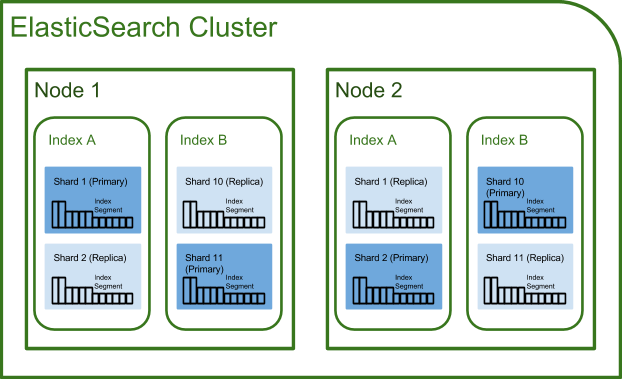
\includegraphics[width=13cm, height=7cm]{images/image_05.png}
\end{center}
\begin{center}
\vspace{0.1cm}
\textbf{Hình 3.} \textit{Kiến trúc Elasticsearch Cluster}    
\end{center}
\vspace{0.3cm}
\textbf{Document} Document là đơn vị cơ bản của dữ liệu trong Elasticsearch hay nói cách khác, dữ liệu trong Elasticsearch được tổ chức thành các document. Document trong Elasticsearch có dạng giống như JSON, bao gồm các thuộc tính và giá trị (giá trị có thể là kiểu String, Long, Boolean, Float,..). Người dùng có thể cấu hình các thuộc tính để bắt buộc có hoặc không bắt buộc, có thể định nghĩa trước hoặc không cần định nghĩa trước. Ví dụ một document trong Elasticsearch:
\begin{center}
\begin{lstlisting}
            {
                "name":         "John Smith",
                "age":          42,
                "confirmed":    true,
                "join_date":    "2014-06-01",
                "home": {
                    "lat":      51.5,
                    "lon":      0.1
                },
                "accounts": [
                    {
                        "type": "facebook",
                        "id":   "johnsmith"
                    },
                    {
                        "type": "twitter",
                        "id":   "johnsmith"
                    }
                ]
            }
\end{lstlisting}
\end{center}
\textbf{Index} Index (chỉ mục) là một tập hợp của các document mà chứa những đặc điểm tương tự. Ví dụ, chúng ta có chỉ mục về dữ liệu khách hàng, một chỉ mục khác về danh mục sản phẩm, và những chỉ mục khác cho những data khác. Chỉ mục cũng được định danh bằng tên, tên này được sử dụng khi thực hiện các hoạt động như lập chỉ mục, tìm kiếm, cập nhật hoặc xóa các document trong đó.

\textbf{Type} Type được sử dụng làm danh mục của một chỉ mục, cho phép lưu trữ các loại dữ liệu khác nhau trong cùng một chỉ mục.

\textbf{Shards \& Replicas}
Một chỉ mục trong Elasticsearch có thể lưu trữ một lượng lớn dữ liệu, thậm chí lớn hơn cả kích cỡ ổ đĩa cứng tại một node. Điều này khiến cho node đó phản hồi chậm với các truy vấn khi lượng dữ liệu tăng. Để giải quyết vấn đề này, Elasticsearch cung cấp khả năng cho phép chia dữ liệu trong một chỉ mục ra thành các phân mảnh nhỏ hơn, gọi là \textit{shard}. Khi tạo mới một chỉ mục, người dùng có thể cấu hình số \textit{shard} mà dữ liệu chỉ mục có thể được chia, nếu không Elasticsearch sẽ để một giá trị mặc định.

Các \textit{shard} có thể được chia ra nhiều node khác nhau, qua đó giảm tải lượng dữ liệu tập trung trên một node khiến node bị quá tải. Ngoài ra, việc chia \textit{shard} như vậy cho phép dữ liệu được lưu trữ phân tán.

Trong một số trường hợp, node bị down hoặc offline, để đảm bảo \textit{high available} cho hệ thống, việc nhân bản dữ liệu là cần thiết. Việc nhân bản dữ liệu trong Elasticsearch được thực hiện bằng việc nhân bản các \textit{shard} và người dùng có thể cấu hình được số lượng nhân bản này. Việc này còn giúp mở rộng kích thước hoặc thông lượng tìm kiếm, bởi các tìm kiếm có thể được thực hiện song song trên các node.

Tóm tắt lại, để có thể lưu trữ dữ liệu phân tán, Elasticsearch chia dữ liệu trong một chỉ mục ra các \textit{shard}, các \textit{shard} này được phân chia ra các node và có thể nhân bản các shard này. Từ đó giúp tăng khả năng chịu tải cũng như tính \textit{available} cho hệ thống.

\subsubsection{Truy vấn trong Elasticsearch}
Elasticsearch hỗ trợ người dùng rất nhiều kiểu truy vấn, hướng tới những mục đích và công việc khác nhau. Trong phạm vi của phần \textit{cơ sở lý thuyết về Elasticsearch}, tôi chỉ giới thiệu những truy vấn tôi sử dụng trong đồ án.
\vspace{0.2cm}
\newline
\textbf{Truy vấn DSL}

\textit{Domain Specific Language (DSL)} - Ngôn ngữ miền chuyên biệt là một ngôn ngữ máy tính, chuyên dùng cho một lĩnh vực, miền ứng dụng cụ thể. Ở đây, Elasticsearch cung cấp truy vấn DSL và dựa trên JSON để định nghĩa các truy vấn. Truy vấn DSL trong Elasticsearch thông thường được chia thành loại chính :

\begin{itemize}
    \item Leaf query clauses : Là truy vấn mà tìm kiếm một giá trị cụ thể trong một trường cụ thể, thường là các query \textit{match, term, range}.
    \item Compound query clauses : Là các truy vấn có thể bao gồm \textit{leaf query clauses} và cả \textit{compound query clauses} khác, thực hiện các truy vấn phức tạp như truy vấn \textit{ bool, dis\_max}. 
\end{itemize}
\textbf{Các truy vấn thông dụng}

\begin{itemize}
    \item Truy vấn \textit{match} : đây là một truy vấn tiêu chuẩn để thực hiện các truy vấn \textit{full text}, bao gồm \textit{fuzzy matching} và truy vấn theo cụm từ hoặc truy vấn gần đúng.  
    \item Truy vấn \textit{match\_phrase} : giống như truy vấn \textit{match} nhưng được sử dụng để tìm kiếm chính xác một cụm từ hoặc một cụm từ với các từ gần đúng.
    \item Truy vấn \textit{bool} : Là một truy vấn cấp cao, thường dùng để kết hợp nhiều truy vấn \textit{leaf query clauses}, cho phép truy vấn phức tạp sử dụng các điều kiện \textit{or, and, not}. \textit{Bool query} hỗ trợ các tham số :
    
        \hspace{1cm} - \textit{must} : phải phù hợp với tất cả các điều kiện và đóng góp vào điểm số, tương đương với \textit{and}.
        
        \hspace{1cm} - \textit{must\_not} : ngược lại với \textit{must}, phải không phù hợp với tất cả các điều kiện, tuơng đuơng với câu lệnh\textit{ not}.
        
        \hspace{1cm} - \textit{should} : phù hợp với một hoặc một vài trong số tất cả các điều kiện, tuơng đuơng với câu lệnh \textit{ or}.
        
        \hspace{1cm} - \textit{minimum\_should\_match} : có kiểu dữ liệu là số nguyên, quy định số kết quả mà \textit{should} bắt buộc phải khớp, mặc định là bằng $1$.
        
\end{itemize}

\section{Các độ đo sử dụng trong bài toán}
\subsection{Độ tương tự Jascard}
Độ tương tự \textit{Jascard} là một chỉ số thống kê, thường được dùng để đánh giá mức độ tương đồng hoặc đa dạng của các tập mẫu với nhau. Độ tương tự \textit{Jascard} được tính bằng cách lấy giao của hai tập hợp chia cho hợp của hai tập hợp:
$$J(A,B) = \frac{|A \cap B|}{|A \cup B|}$$
\begin{center}

\vspace{0.1cm}
\textbf{3.15.} \textit{Độ đo Jascard}    
\end{center}
Trong đó $A, B$ là hai tập hữu hạn. Trong trường hợp cả hai tập đều rỗng, thì $J(A,B) = 0$. Vậy nên :
$$0 \leq J(A,B) \leq 1$$

\subsection{Khoảng cách Levenshtein}

